
\section{Experiments}
\FloatBarrier
When dealing with neural networks there are a wide range of network structures and optimization algorithms. An in depth search for the best parameters will not be the focus of this chapter. The main focus of this chapter will be to investigate when reparametrization by neural networks is possible.

We also investigate whether the deviation from the optimal solution is optimization error or approximation error.  Thus by the results in chapter [0] we investigate how increasing the network size impacts the resulting error. This approach will still be somewhat ambiguous; since increasing the networks size simultaneously increases the dimension of the optimization problem. Also with increasing layers we have the vanishing gradient problem.[0]

\subsection{Curves from the same shape}
\FloatBarrier
In this experiment we used the example from \cite[Section 4.2.6]{jørgen2021}. The SRVT was not used in the original experiment, but SRV form of the two curves considered are the same. Thus, we considered a curve with SRV form \(r\) given by 
\begin{equation*}
    r(t) = \pi [-2 \sin(2\pi t), 4\cos(4\pi t)]^T,
\end{equation*}
and its reparametrization \(q = \sqrt{\psi'}q \circ \psi\), where 
\begin{equation*}
    \psi(t) = \frac{\log(20t + 1)}{2 \log(21)} + \frac{\tanh(20(t - 0.5))}{4 \tanh(10)}.
\end{equation*}
The SRV form of the curves is shown in Figure \ref{fig:curve_1}. 

\begin{figure}[b]
    % \begin{subfigure}[b]{0.5\textwidth}\label{fig:curve_1_c_1}
    %     \centering
    %     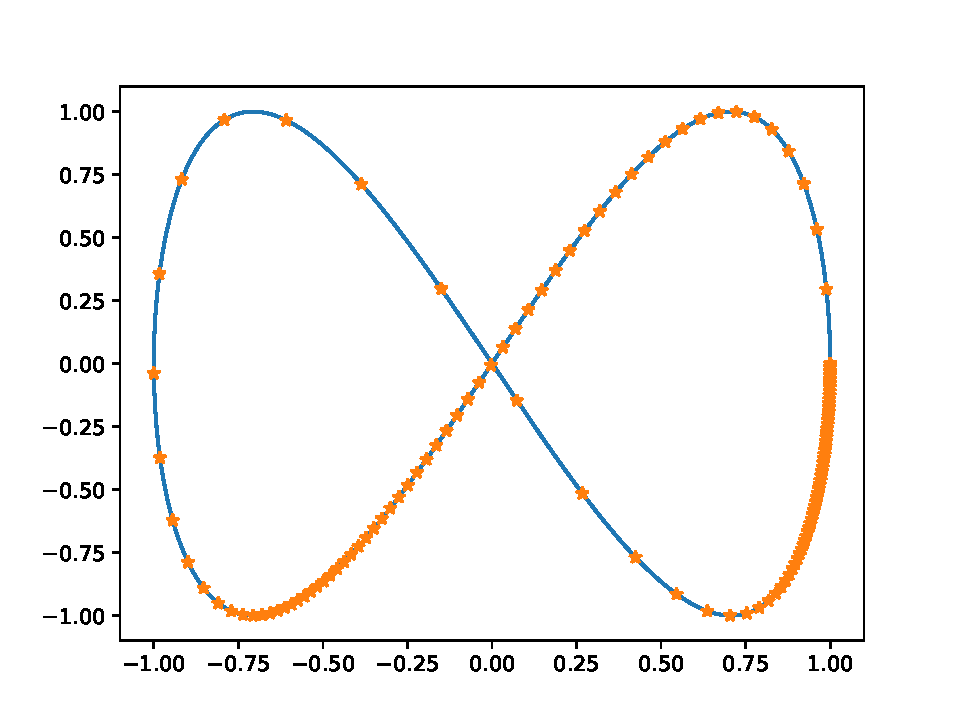
\includegraphics[width=\linewidth]{figures/curve_1/curve_c_1.pdf}
    %     \caption{\(c_1\)}
    % \end{subfigure}
    % \begin{subfigure}[b]{0.5\textwidth}\label{fig:curve_1_c_2}
    %     \centering
    %     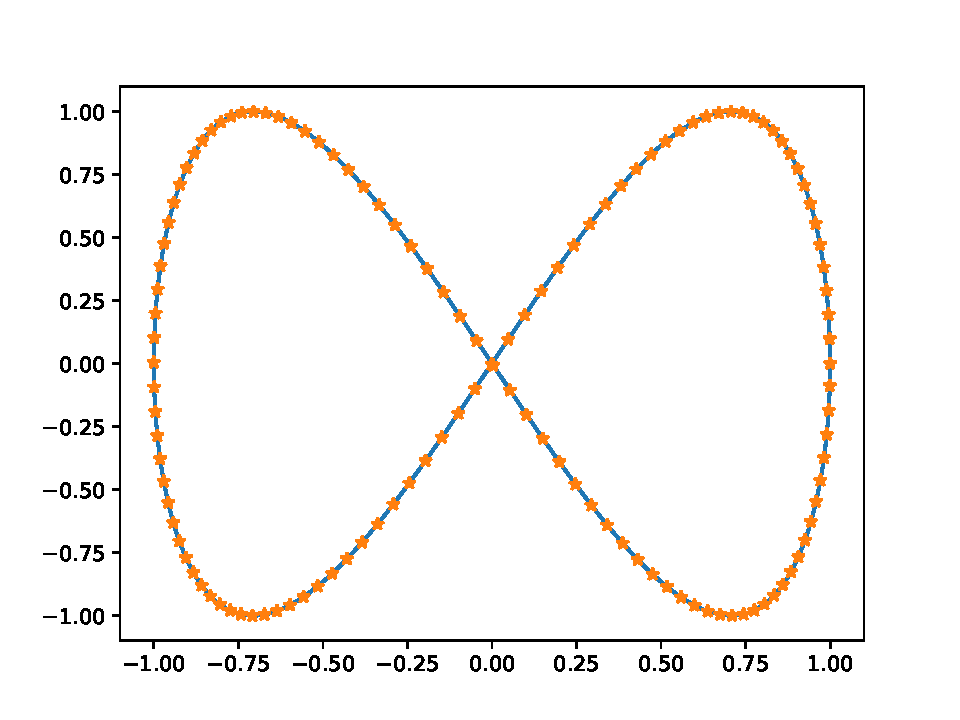
\includegraphics[width=\linewidth]{figures/curve_1/curve_c_2.pdf}
    %     \caption{\(c_2\)}
    % \end{subfigure}
    \begin{subfigure}[t]{0.5\textwidth}
        \centering
        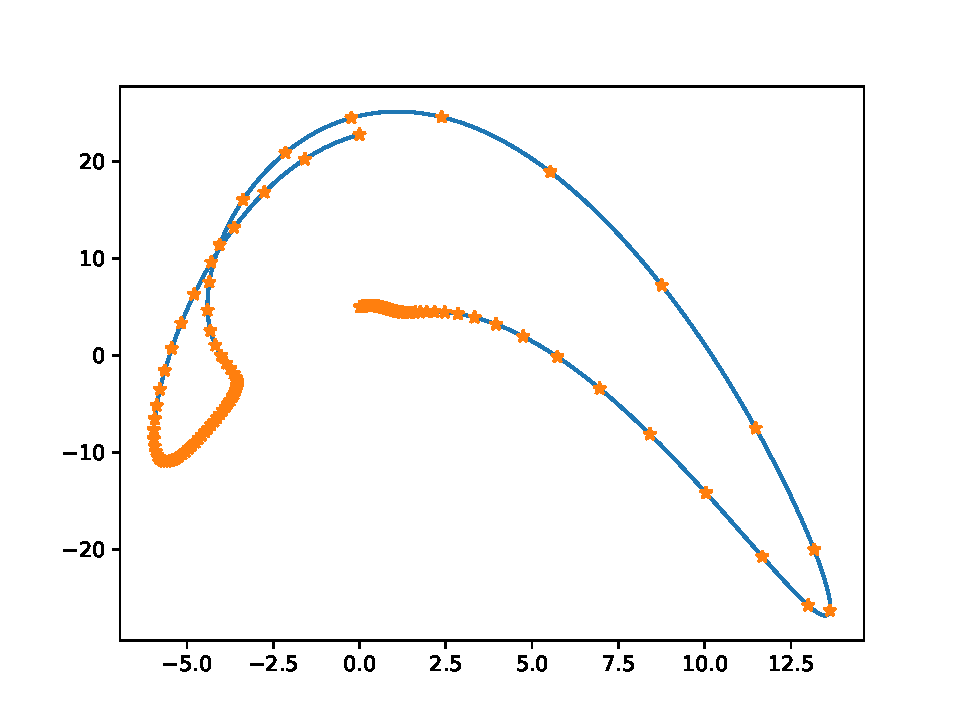
\includegraphics[width=\linewidth]{figures/curve_1/curve_q.pdf}
        \caption{\(q\)}\label{fig:curve_1_q}
    \end{subfigure}
    \begin{subfigure}[t]{0.5\textwidth}
        \centering
        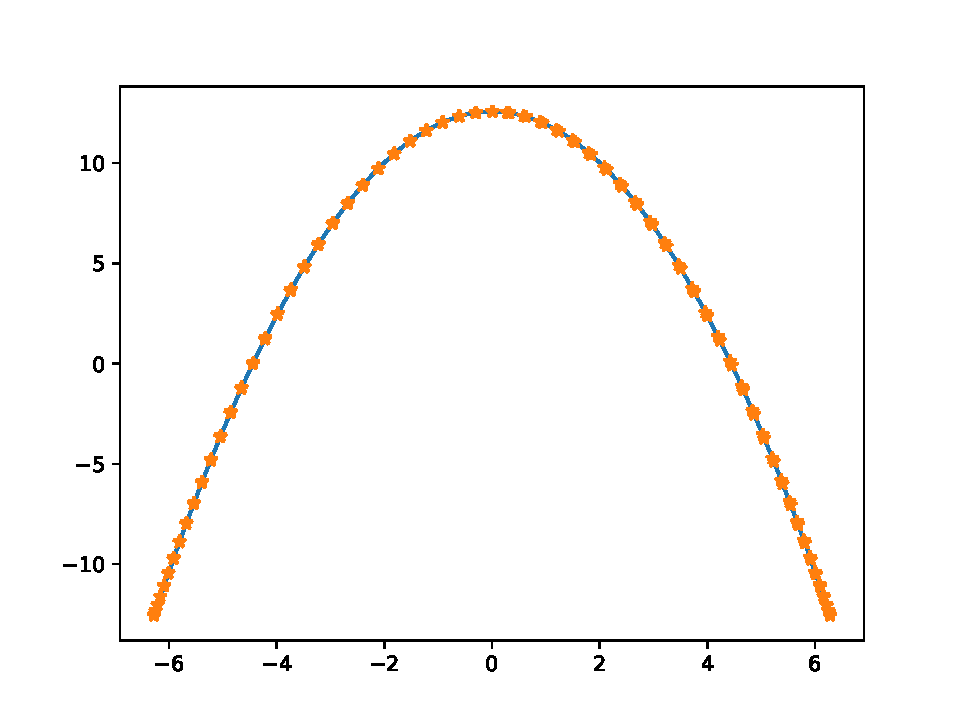
\includegraphics[width=\linewidth]{figures/curve_1/curve_r.pdf}
        \caption{\(r\)}\label{fig:curve_1_r}
    \end{subfigure}
    \caption{The trajectories of \(q\) and \(r\) which are the SRV form defined by the problem in Subsection \ref{subsec:case_1}}\label{fig:curve_1}
\end{figure}


\begin{figure}
    \begin{subfigure}[t]{0.5\textwidth}
        \centering
        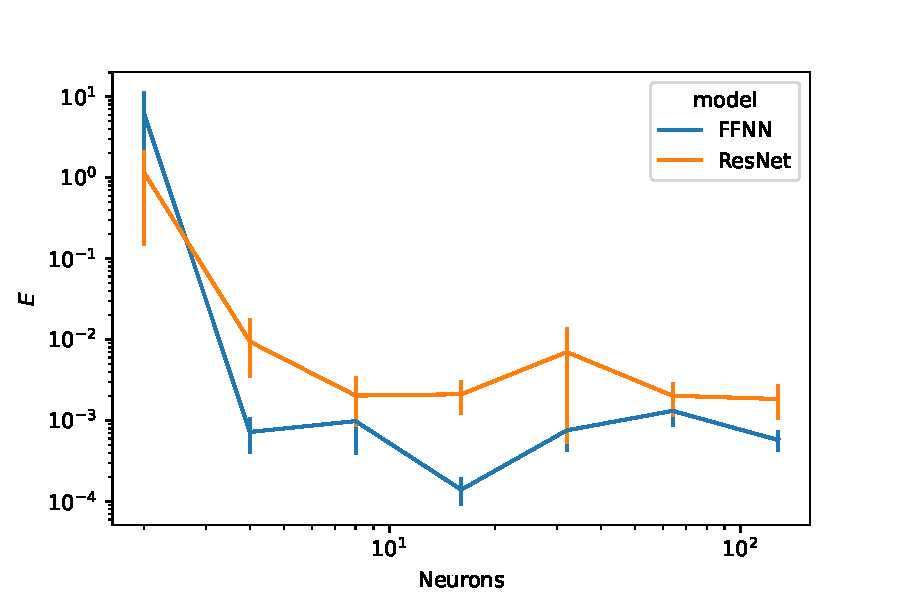
\includegraphics[width=\linewidth]{figures/curve_1/eks_7/neurons_error.pdf}
        \caption{The final cost \(E\) with the number of neurons in each hidden layer.} \label{fig:curve_1_neuron_error} \end{subfigure}
    \begin{subfigure}[t]{0.5\textwidth}
        \centering
        \includegraphics[width=\linewidth]{figures/curve_1/eks_7/layer_error.pdf}
        \caption{Final cost \(E\) with the number of hidden layers.} \label{fig:curve_1_layer_error}
    \end{subfigure}
    \caption{Result of ensemble training with different number of neurons and hidden layers. In Figure \ref{fig:curve_1_neuron_error} the number of layers was fixed at 2. In Figure \ref{fig:curve_1_layer_error} the number of neurons is fixed at 8 per hidden layer. The error bars denote a 80\% confidence interval found by bootstrapping.} \label{fig:curve_1_parmas_eks}
\end{figure}

\begin{figure}[b]
    \begin{subfigure}[t]{0.5\textwidth}
        \centering
        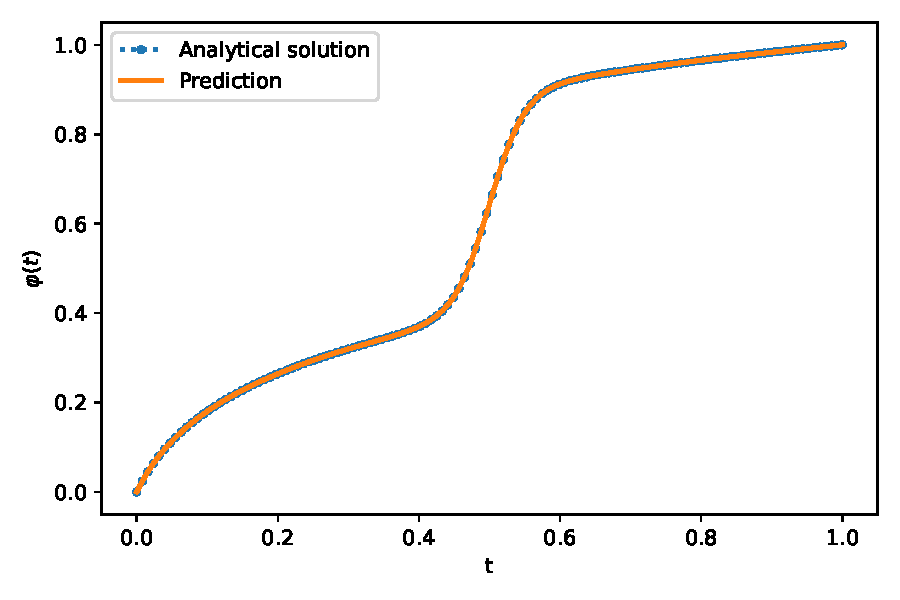
\includegraphics[width=\linewidth]{figures/curve_1/eks_7/plot_2_0.pdf}
        \caption{The approximate optimal reparametrization and the analytical solution.}\label{fig:curve_1_solution}
    \end{subfigure}
    \begin{subfigure}[t]{0.5\textwidth}
        \centering
        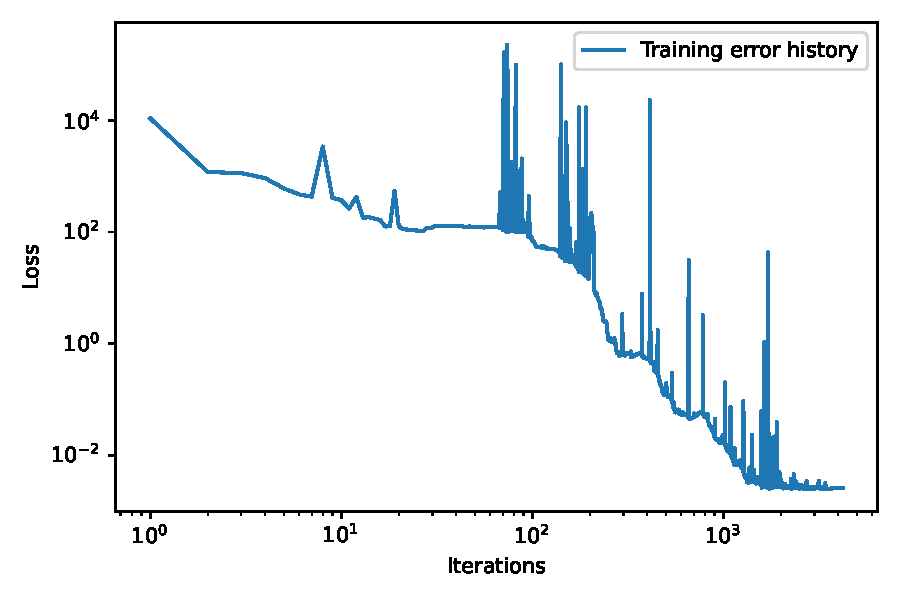
\includegraphics[width=\linewidth]{figures/curve_1/eks_7/history_plot_2.pdf}
        \caption{The cost function \(\mathcal{J}(\theta)\) with each iteration.}\label{fig:curve_1_history}
    \end{subfigure}
    \caption{Result of one optimization procedure with the corresponding loss history.}\label{fig:curve_1_example}
\end{figure}


We performed ensemble training with different network structures, lengths, and widths to test how our method performs on the problem. An overview of the result is shown in Figure \ref{fig:curve_1_parmas_eks}. Moreover, the resulting optimal reparametrization of the first training procedure can be seen in Figure \ref{fig:curve_1_example}. One possible observation is that a ResNet structure permits the training of deeper neural networks better than fully connected feedforward networks.

Reparametrization by neural networks was also compared to deep reparametrization. The comparison was made with respect to the cost function \(\hat E\), as defined in \eqref{eq:discretized_cost}, and is shown in Table \ref{tab:comare_res_palais}. We see that deep reparametrization outperforms our method significantly for this problem. Moreover, deep reparametrization produced the same solution for each training. This is not the case for reparametrization by neural networks since the initial condition \(\theta_0\) is random.
\begin{table}[b]
    \centering
    \begin{tabular}{lrl}
        \toprule
        \(\hat{E} \) & Degrees of freedom & Model         \\
        \midrule
        0.002212     & 33                 & ResNet        \\
        0.000676     & 2257               & ResNet        \\
        0.004567     & 30                 & Deep reparametrization \\
        0.000002     & 10000              & Deep reparametrization\\
        \bottomrule
    \end{tabular}
    \caption{Comparison of the performance of reparametrization by residual neural network and deep reparametrization. Each experiment is the average of the same optimization procedure. Deep reparametrization was performed using. Here the degrees is meant as the number of trainable parameters in the model.}\label{tab:comare_res_palais}
\end{table}


\FloatBarrier
\subsection{Curves from different shapes}
\begin{figure}[t]\label{fig:curve_2}
    \begin{subfigure}[b]{0.5\textwidth}\label{fig:curve_2_c_1}
        \centering
        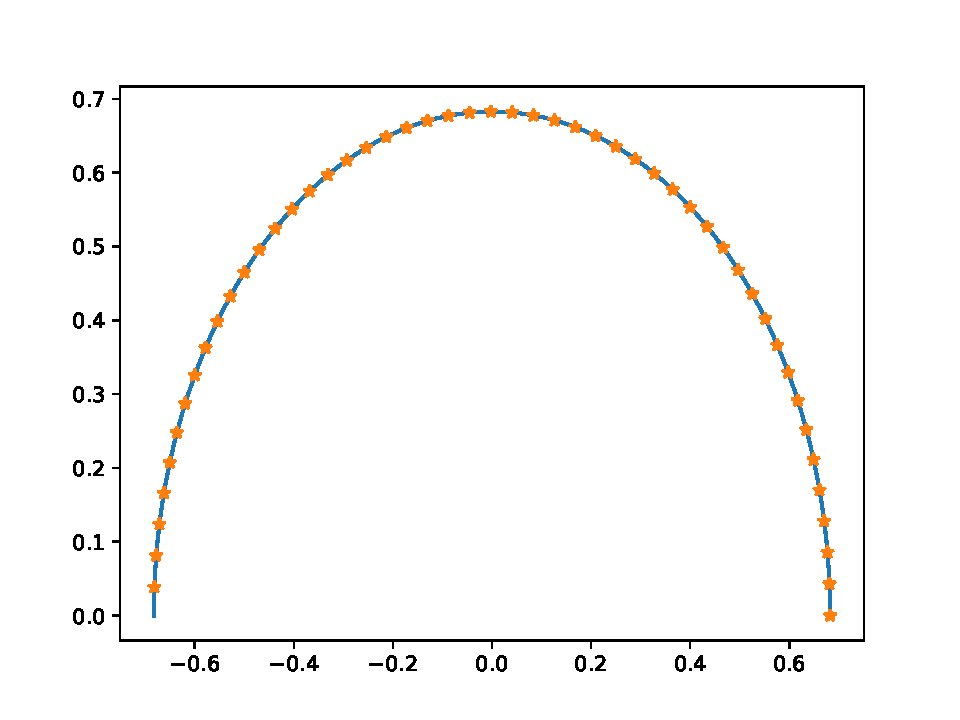
\includegraphics[width=\linewidth]{figures/curve_2/curve_c_1.pdf}
        \caption{\(c_1\)}
    \end{subfigure}
    \begin{subfigure}[b]{0.5\textwidth}\label{fig:curve_2_c_2}
        \centering
        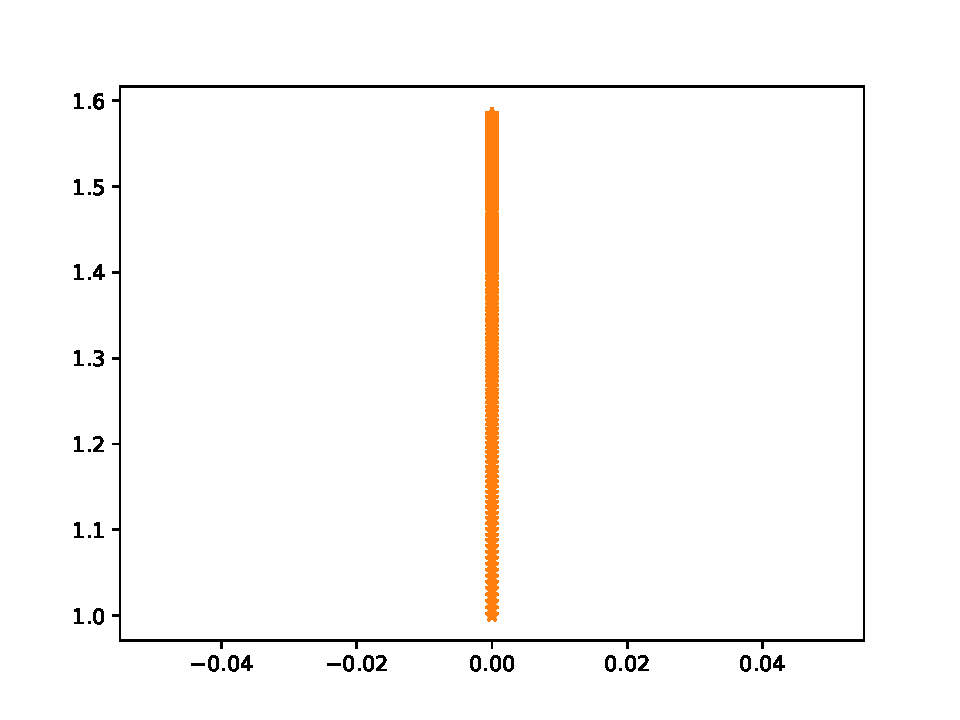
\includegraphics[width=\linewidth]{figures/curve_2/curve_c_2.pdf}
        \caption{\(c_2\)}
    \end{subfigure}
    \begin{subfigure}[t]{0.5\textwidth}\label{fig:curve_2_q}
        \centering
        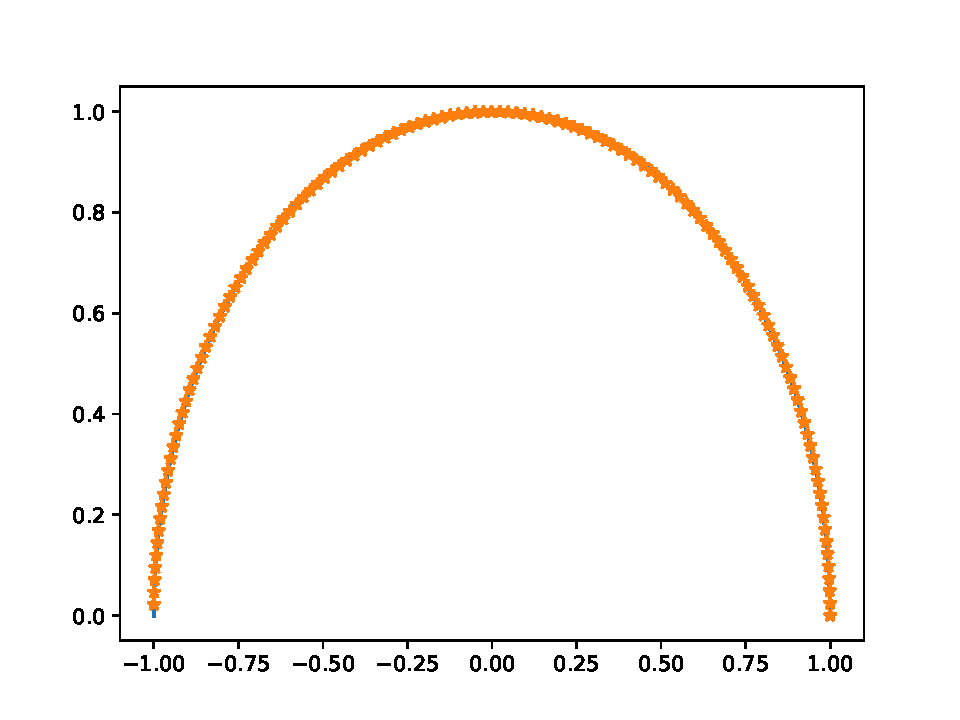
\includegraphics[width=\linewidth]{figures/curve_2/curve_q.pdf}
        \caption{\(q\)}
    \end{subfigure}
    \begin{subfigure}[t]{0.5\textwidth}\label{fig:curve_2_r}
        \centering
        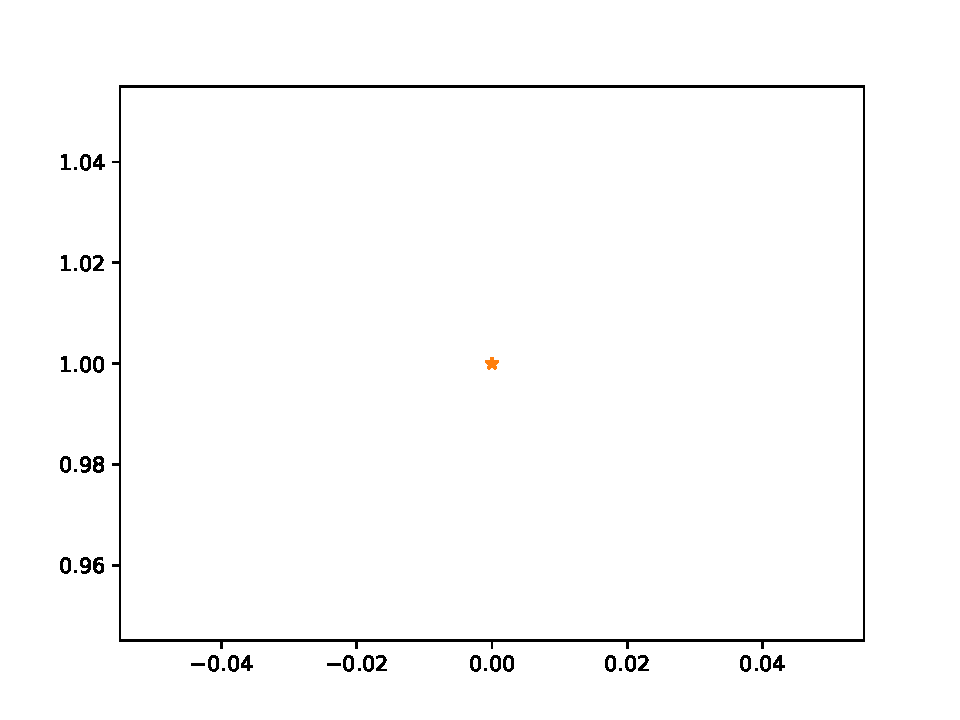
\includegraphics[width=\linewidth]{figures/curve_2/curve_r.pdf}
        \caption{\(r\)}
    \end{subfigure}
    \caption{The trajectory of \(c_1, c_2 \in \text{Imm}(I, \R^2)\), \(q = Q(c_1)\) and \(r = Q(c_2)\).}
\end{figure}

\begin{figure}[t]\label{fig:curve_2_example}
    \begin{subfigure}[t]{0.5\textwidth}\label{fig:curve_2_solution}
        \centering
        \includegraphics[width=\linewidth]{figures/curve_2/curve_2_exp_2/curve_2_exp_2_1_0.pdf}
        \caption{The approximate optimal reparametrization and the analytical solution.}
    \end{subfigure}
    \begin{subfigure}[t]{0.5\textwidth}\label{fig:curve_2_history}
        \centering
        \includegraphics[width=\linewidth]{figures/curve_2/curve_2_exp_2/history_curve_2_exp_2_0.pdf}
        \caption{The cost function \(L(\theta)\) with each iteration.}
    \end{subfigure}
    \caption{The approximate solution to test problem (2) found by a neural network and the corresponding loss history.}
\end{figure}

\begin{figure}[t]\label{fig:curve_2_parmas_eks}
    \begin{subfigure}[t]{0.5\textwidth}
        \centering
        \includegraphics[width=\linewidth]{figures/curve_2/curve_2_exp_2/neurons_error.pdf}
        \caption{The final cost \(E\) with the number of neurons in each hidden layer.}
        \label{fig:curve_2_neuron_error}
    \end{subfigure}
    \begin{subfigure}[t]{0.5\textwidth}
        \centering
        \includegraphics[width=\linewidth]{figures/curve_2/curve_2_exp_2/layer_error.pdf}
        \caption{Final cost \(E\) with the number of layers.}
        \label{fig:curve_2_layer_error}
    \end{subfigure}
    \caption{Result of ensemble training for test problem (2) with different number of neurons and hidden layers. In Figure \ref{fig:curve_2_neuron_error} the number of layers was fixed at 2. In Figure \ref{fig:curve_2_layer_error} the number of neurons is fixed at 8 per hidden layer. The error bars denote a 80\% confidence interval found by bootstrapping.}
\end{figure}


Better structures and optimization algoritmhs for deeper networks.


\FloatBarrier
\subsection{Piecewise linear and piecewise constant}

\begin{figure}[t]\label{fig:curve_1_pc}
    \begin{subfigure}[t]{0.5\textwidth}\label{fig:curve_1_pc_q}
        \centering
        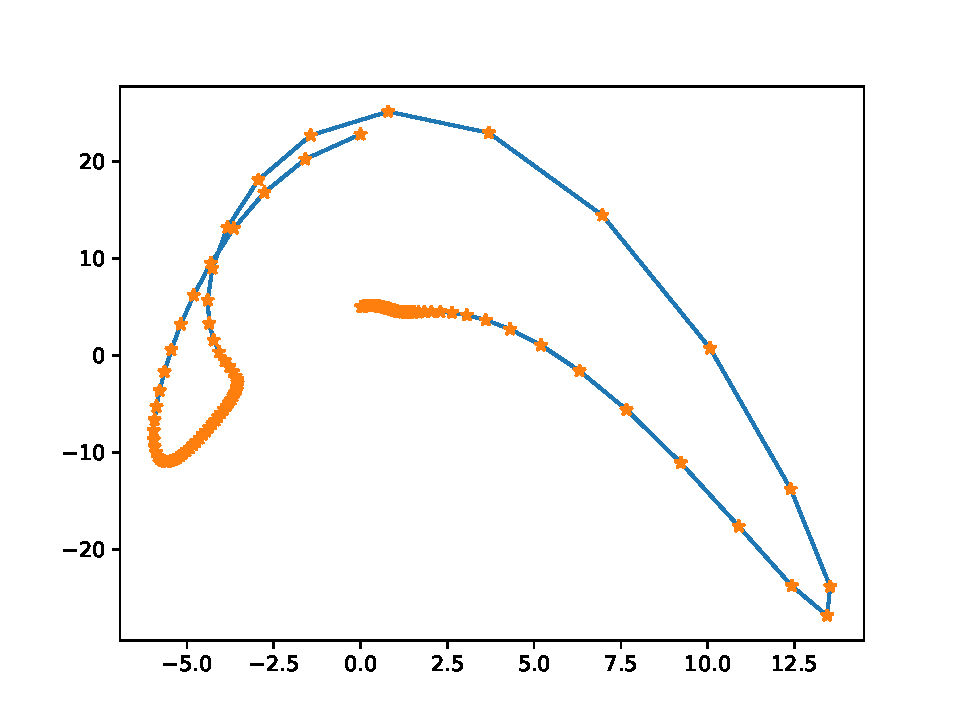
\includegraphics[width=\linewidth]{figures/curve_1/curve_q_pc.pdf}
        \caption{\(\bar q\)}
    \end{subfigure}
    \begin{subfigure}[t]{0.5\textwidth}\label{fig:curve_1_pc_r}
        \centering
        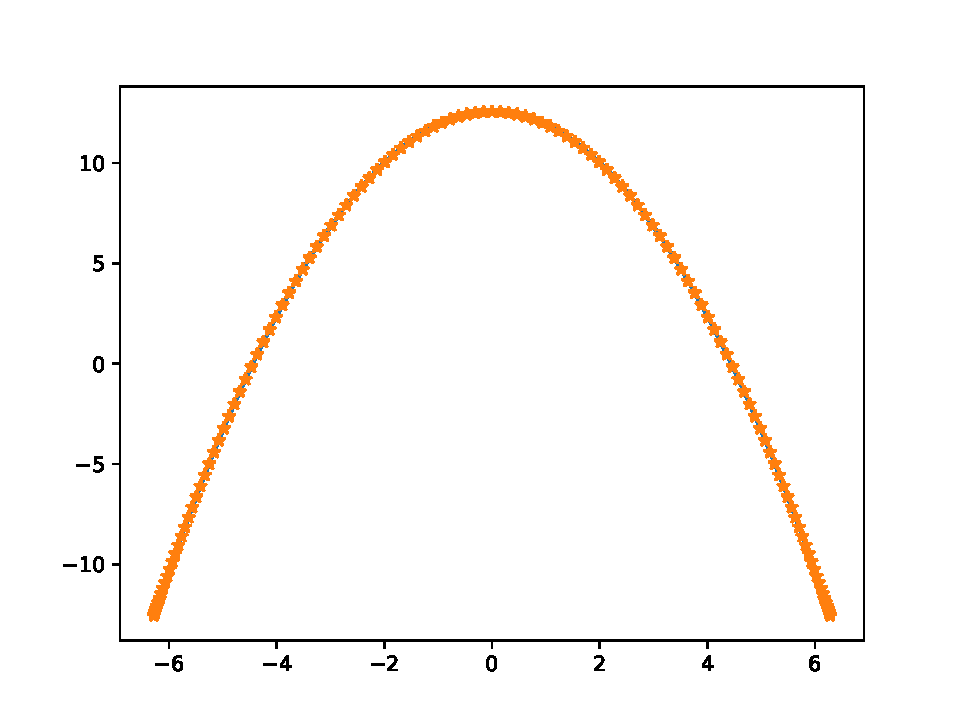
\includegraphics[width=\linewidth]{figures/curve_1/curve_r_pc.pdf}
        \caption{\(\bar r\)}
    \end{subfigure}
    \caption{The trajectory of \(\bar q\) and \(\bar r\) being piecewise constant interpolations of $q$ and $r$ from test problem (1).}
\end{figure}

\begin{figure}[t]\label{fig:curve_1_pc_pl_example}
    \begin{subfigure}[t]{0.5\textwidth}
        \centering
        \includegraphics[width=\linewidth]{figures/curve_1_pc/curve_pc_1/curve_pc_1_0_0.pdf}
        \caption{The approximate optimal reparametrization and the analytical solution.}
        \label{fig:curve_1_pc_solution}
    \end{subfigure}
    \begin{subfigure}[t]{0.5\textwidth}
        \centering
        \includegraphics[width=\linewidth]{figures/curve_1_pc/curve_pc_1/history_curve_pc_1_0.pdf}
        \caption{The cost function \(L(\theta)\) with each iteration.}
        \label{fig:curve_1_pc_history}
    \end{subfigure}
    \begin{subfigure}[t]{0.5\textwidth}
        \centering
        \includegraphics[width=\linewidth]{figures/curve_1_pl/curve_1_pl_exp_1/curve_1_pl_exp_1_1_0.pdf}
        \caption{The approximate optimal reparametrization and the analytical solution.}
        \label{fig:curve_1_pl_solution}
    \end{subfigure}
    \begin{subfigure}[t]{0.5\textwidth}
        \centering
        \includegraphics[width=\linewidth]{figures/curve_1_pl/curve_1_pl_exp_1/history_curve_1_pl_exp_1_1.pdf}
        \caption{The cost function \(L(\theta)\) with each iteration.}
        \label{fig:curve_1_pl_history}
    \end{subfigure}
    \caption{The approximate solutions to the piecewise constant (\ref{fig:curve_1_pc_solution}) and piecewise linear (\ref{fig:curve_1_pl_solution}) version of test problem (1). The approximate solution is compared to the analytical solution of test problem (1) and the corresponding training history is shown in the figure to the right.}
\end{figure}

\begin{figure}[t]\label{fig:curve_1_pl_eks}
    \begin{subfigure}[t]{0.5\textwidth}
        \centering
        \includegraphics[width=\linewidth]{figures/curve_1_pl/curve_1_pl_exp_1/neurons_error.pdf}
        \caption{The final cost \(E\) with the number of neurons in each hidden layer.}
        \label{fig:curve_1_pl_neuron_error}
    \end{subfigure}
    \begin{subfigure}[t]{0.5\textwidth}
        \centering
        \includegraphics[width=\linewidth]{figures/curve_1_pl/curve_1_pl_exp_1/layer_error.pdf}
        \caption{Final cost \(E\) with the number of layers.}
        \label{fig:curve_1_pl_layer_error}
    \end{subfigure}
    \caption{Result of ensemble training for the piecewise linear version of test problem (1) with different number of neurons and hidden layers. In Figure \ref{fig:curve_2_neuron_error} the number of layers was fixed at 2. In Figure \ref{fig:curve_2_layer_error} the number of neurons is fixed at 8 per hidden layer. The error bars denote a 80\% confidence interval found by bootstrapping.}
\end{figure}

Training of
Error convergence example 

\FloatBarrier
\subsection{Interpolated motion capture data}
In the following experiments, we used two motions from the CMU Graphics Lab Motion Capture Database \cite{mocap}. As seen in subsection \ref{subsec:shape-lie}, motion capture data can be interpolated such that the SRV form is piecewise constant. As in the previous section, these SRV curves were then interpolated by a piecewise linear interpolation. The interpolated curves were then used instead of the original curves in the optimization procedure. As seen in Figure \ref{fig:curve_1_so3_example} the interpolated problem produced an in optimal reparametrization that agreed with the solution given by dynamic programming, implemented by \citeauthor{lystad2019}\cite{lystad2019}. 

\begin{figure}[t]
    \begin{subfigure}[t]{0.5\textwidth}
        \centering
        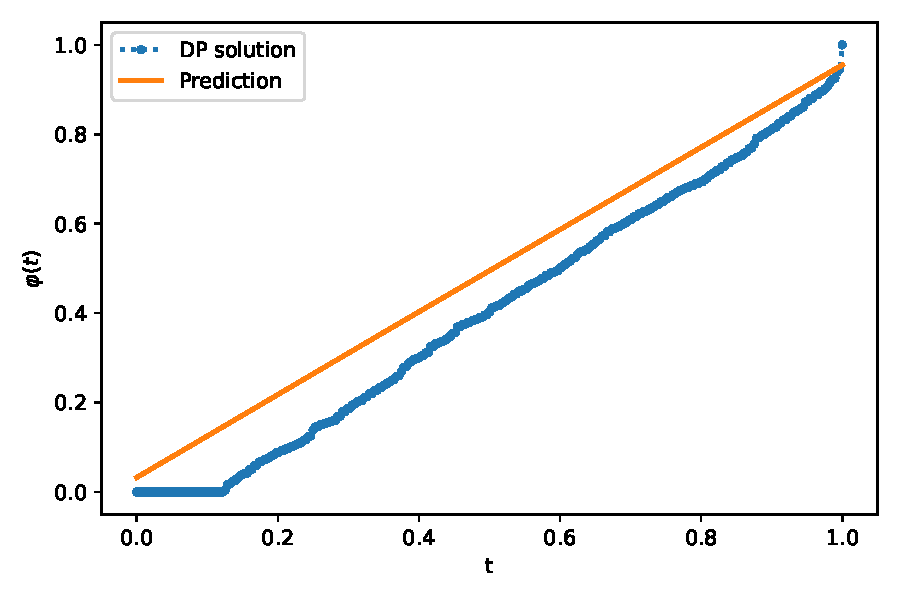
\includegraphics[width=\linewidth]{figures/curve_so3/pc_eks_2/plot_1_0.pdf}
        \caption{Solutions found by neural network training and dynamic programming.}\label{fig:curve_so3_pc_solution}
    \end{subfigure}a
    \begin{subfigure}[t]{0.5\textwidth}
        \centering
        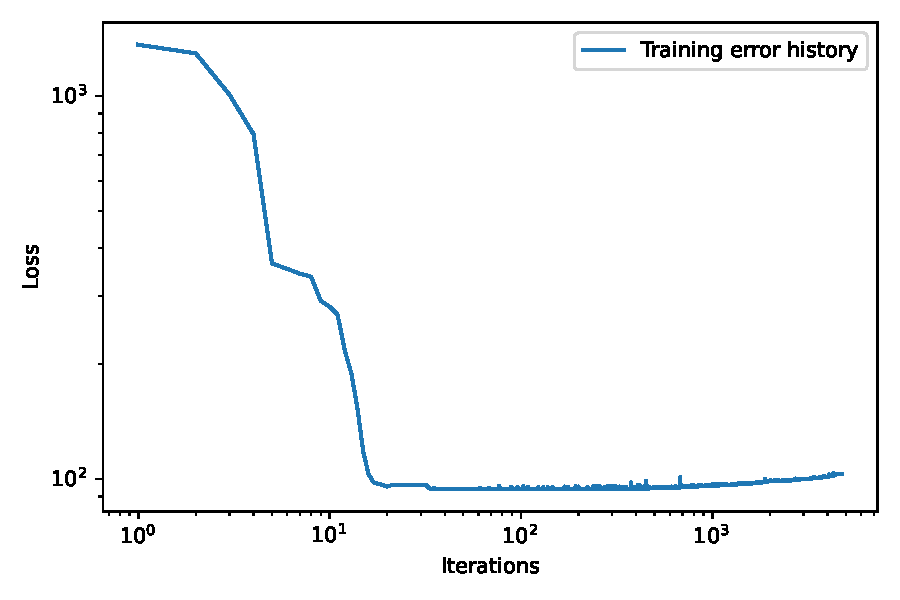
\includegraphics[width=\linewidth]{figures/curve_so3/pc_eks_2/history_plot_1.pdf}
        \caption{The cost function \(L(\theta)\) with each iteration.}\label{fig:curve_so3_pc_history}
    \end{subfigure}
    \begin{subfigure}[t]{0.5\textwidth}
        \centering
        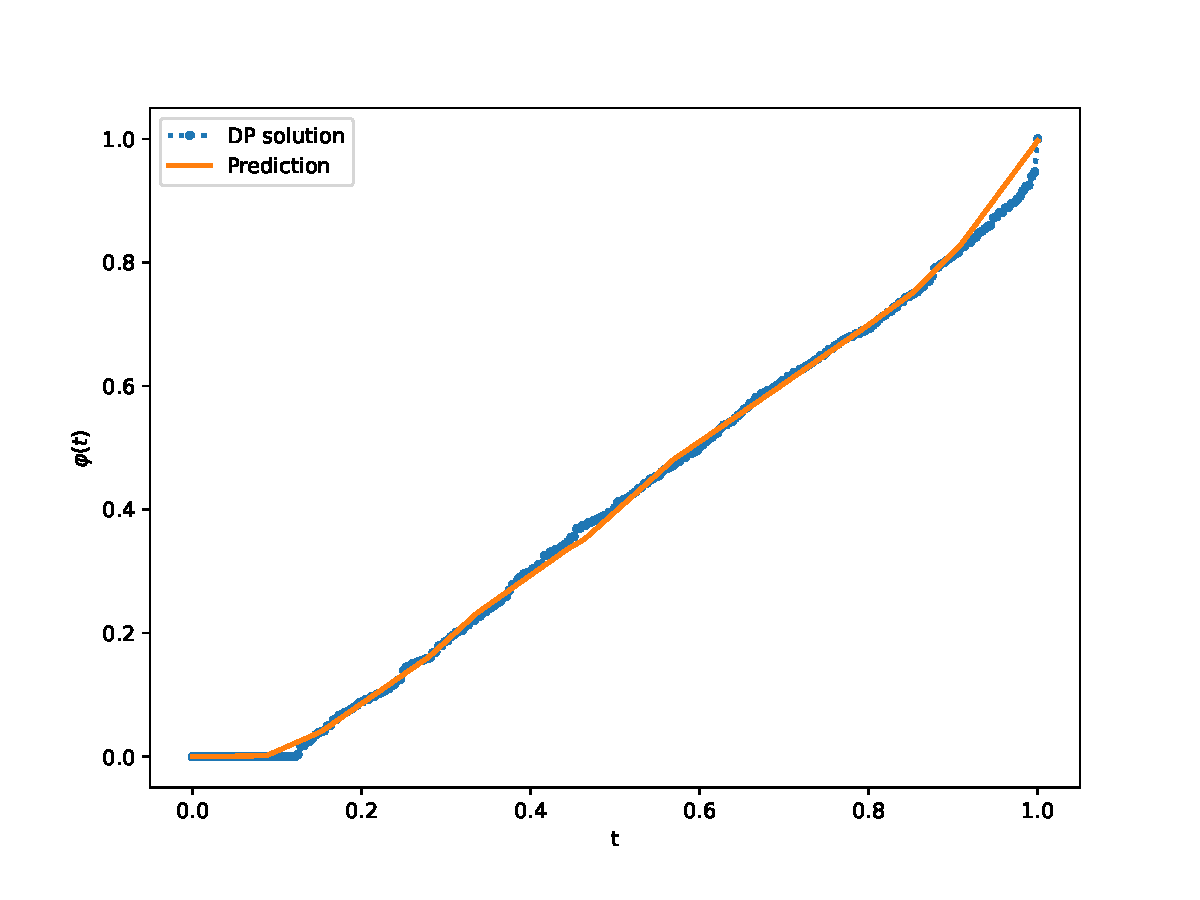
\includegraphics[width=\linewidth]{figures/curve_so3/pl_eks_6/plot_288_0.pdf}
        \caption{Solutions found by neural network training and dynamic programming.}\label{fig:curve_so3_pl_solution}
    \end{subfigure}
    \begin{subfigure}[t]{0.5\textwidth}
        \centering
        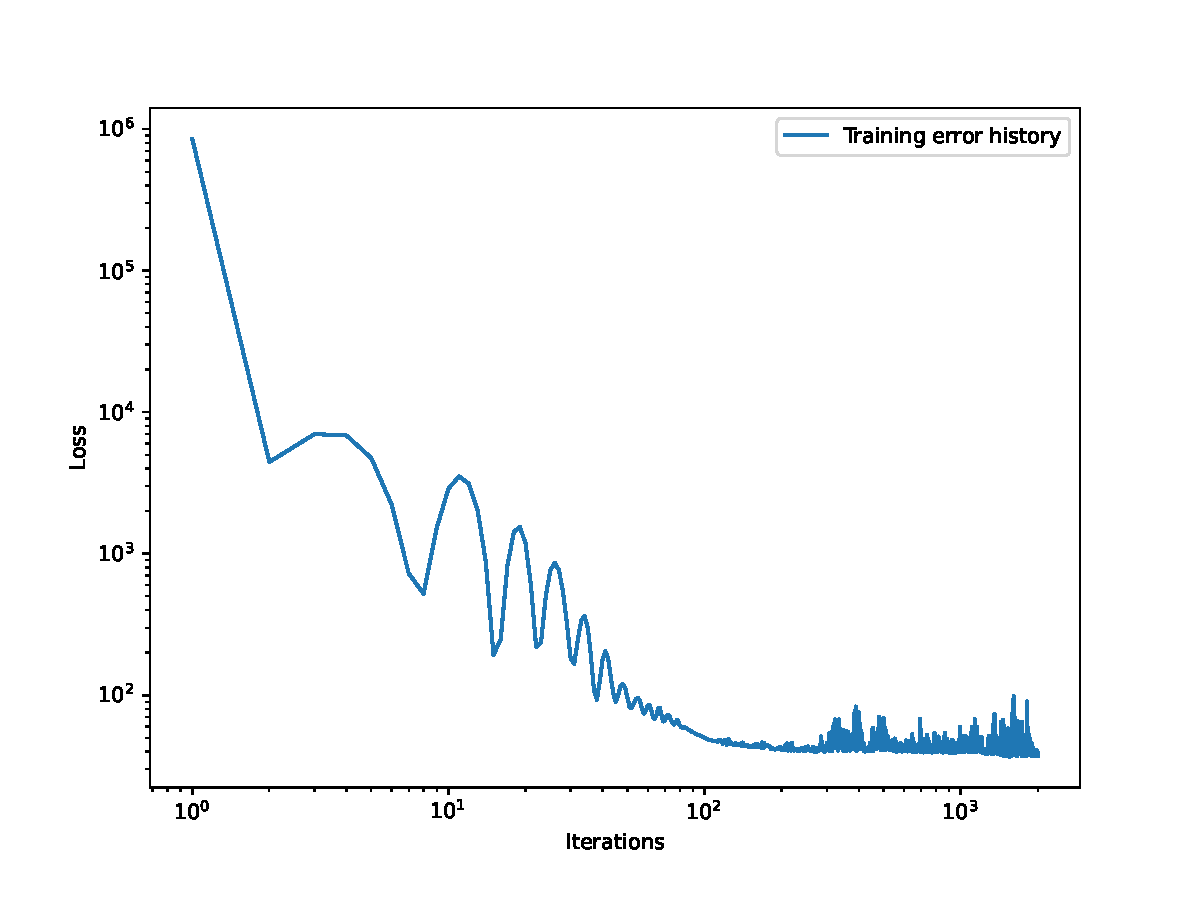
\includegraphics[width=\linewidth]{figures/curve_so3/pl_eks_6/history_plot_288.pdf}
        \caption{The cost function \(L(\theta)\) with each iteration.}\label{fig:curve_so3_pl_history}
    \end{subfigure}
    \caption{The approximate optimal reparametrizations of two curves representing motion capture data. Figure \ref{fig:curve_so3_pc_solution} shows the solution for the original curves, and Figure \ref{fig:curve_so3_pl_solution} shows the solution for the linearly interpolated curve. The approximate solutions are compared to the solution found by a dynamic programming algorithm and the corresponding training history is shown in the figure to the right. }\label{fig:curve_1_so3_example}
\end{figure}

Ensemble training was again performed to observe how the optimal reparametrization is affected by different parameters. The ensemble training result is shown in Figure \ref{fig:curve_so3_pl_eks}. In this experiment, the network structure was not varied. Instead, the performance of ReLU and \(\tanh\) activation function was compared. 

\begin{figure}[t]
    \begin{subfigure}[t]{0.5\textwidth}
        \centering
        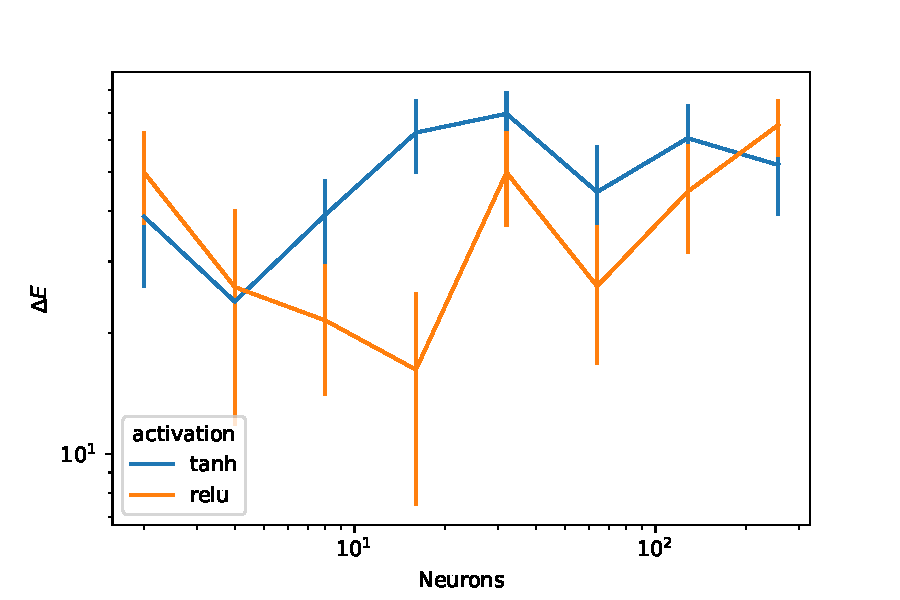
\includegraphics[width=\linewidth]{figures/curve_so3/pl_eks_6/neurons_error.pdf}
        \caption{The final cost \(E\) with the number of neurons in each hidden layer.}\label{fig:curve_so3_pl_neuron_error}
    \end{subfigure}
    \begin{subfigure}[t]{0.5\textwidth}
        \centering
        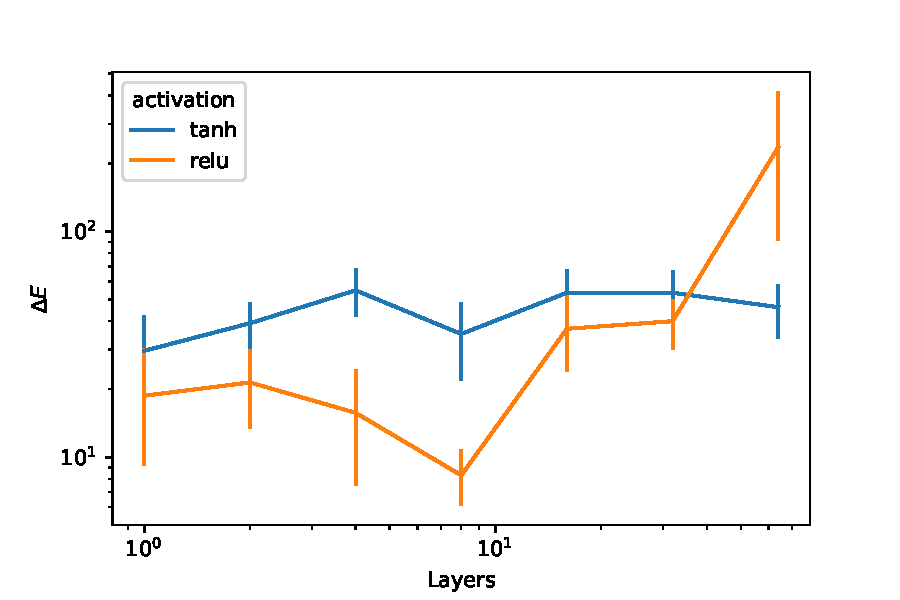
\includegraphics[width=\linewidth]{figures/curve_so3/pl_eks_6/layer_error.pdf}
        \caption{Final cost \(E\) with the number of layers.}\label{fig:curve_so3_pl_layer_error}
    \end{subfigure}
    \caption{Result of ensemble training for the piecewise linear version of the problem with curves generated by motion capture data with different number of neurons and hidden layers. Figure \ref{fig:curve_2_neuron_error} the number of layers was fixed at 2. In Figure \ref{fig:curve_2_layer_error} the number of neurons is fixed at 8 per hidden layer. The error bars denote a 80\% confidence interval found by bootstrapping.}\label{fig:curve_so3_pl_eks}
\end{figure}


